\cleardoublepage
\chapter{Empf�nger}\label{chap:receiver}
\thispagestyle{empty}

\section{Aufbau}\label{sec:receiver:structure}

$\overline{H}$

\begin{figure}[ht]
	\centering 
%	\psfrag{06}{$N$}
	\includegraphics[width=10cm]{bilder/empfaenger/Empf�ngerstufe}
	\caption{Blockschaltbild der Empf�ngerstufe}
	\label{fig:Empf�nger}
\end{figure}

Der Empf�nger ist aus zwei identischen Zweigen aufgebaut. Jeder Zweig besteht, wie in Abb. \ref{fig:Empf�nger} dargestellt, aus einem Bandpass\index{Bandpass}, einem H�llkurvendemodulator\index{H�llkurvendemodulator} und einem Tiefpass\index{Tiefpass}. Am Eingang wird das FSK-modulierte Signal (vgl. Abb. \ref{fig:Sendesig} des Senders) eingespeist und auf die beiden Empfangszweige\index{Empfangszweige} aufgeteilt.

\begin{figure}[ht]
	\centering 
%	\psfrag{06}{$N$}
	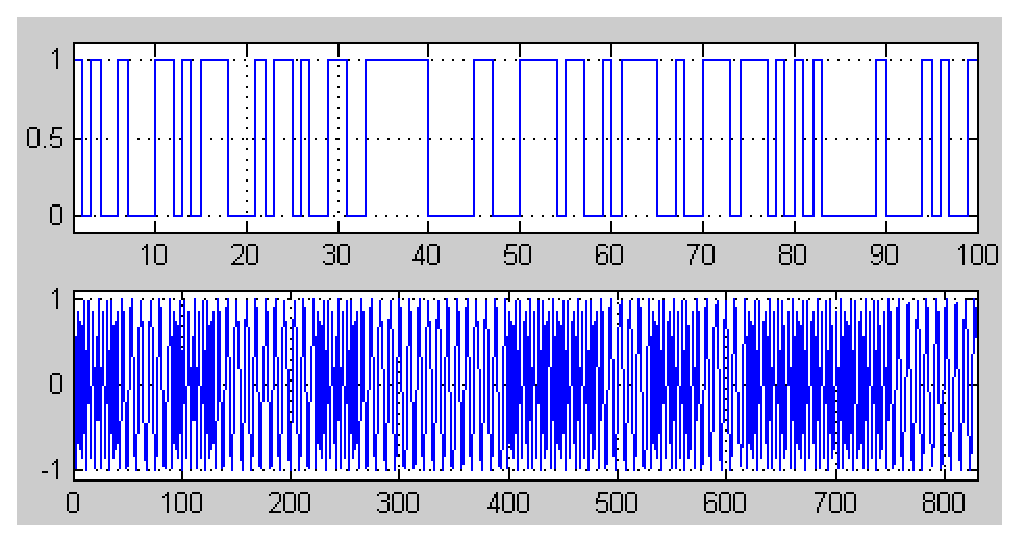
\includegraphics[width=8cm]{bilder/empfaenger/Sendesig}
	\caption{Bitstrom und Sendesignal}
	\label{fig:Sendesig}
\end{figure}

Jeder Bandpass hat die Aufgabe, eine der beiden Signalfrequenzen zu separieren, so dass pro Zweig nur noch eine einzige Frequenz detektiert werden kann. Somit liefert also in einem Zweig nur noch die der Null zugeordnete Frequenz einen Beitrag, im anderen Zweig die der Eins zugeordnete Frequenz. Dies ist in Abbildung \ref{fig:Bandpassig} dargestellt.

\begin{figure}[ht]
	\centering 
%	\psfrag{06}{$N$}
	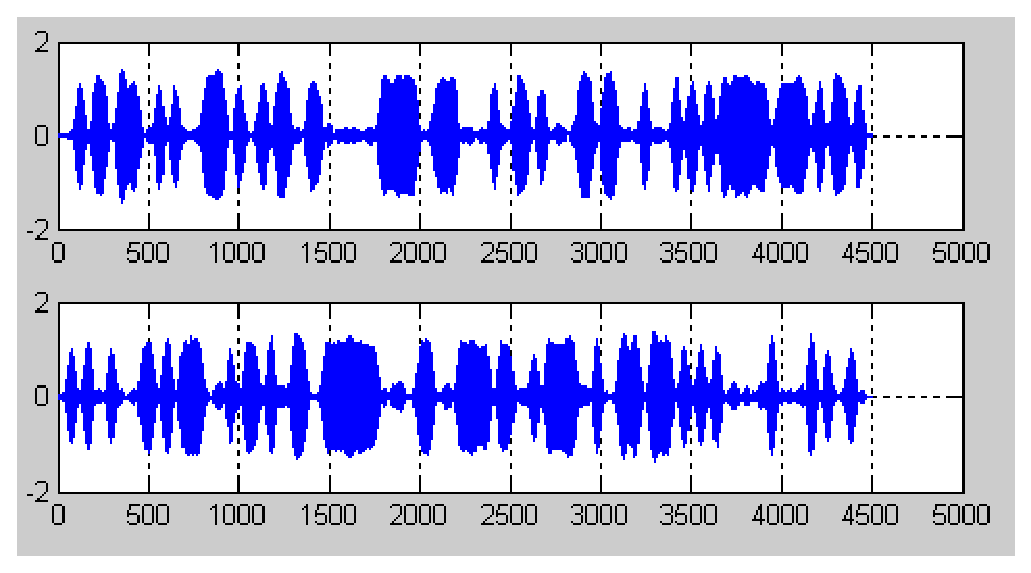
\includegraphics[width=8cm]{bilder/empfaenger/Bandpassgef}
	\caption{Bandpassgefilterte Signale}
	\label{fig:Bandpassig}
\end{figure}

Um nun wieder ein eindeutiges Signal zu erhalten, wird eine H�llkurven\-demodulation durchgef�hrt. Hier wird durch eine einfache Quadrierung des Signals die negative Halbwelle des Sinussignals nach oben ``geklappt'' (vgl. Abb. \ref{fig:Quadriertessig}) und danach mit einem Tiefpass gegl�ttet. Das Ergebnis ist in Abb. \ref{fig:quadutpgefsig} dargestellt.

\begin{figure}[ht]
	\centering 
%	\psfrag{06}{$N$}
	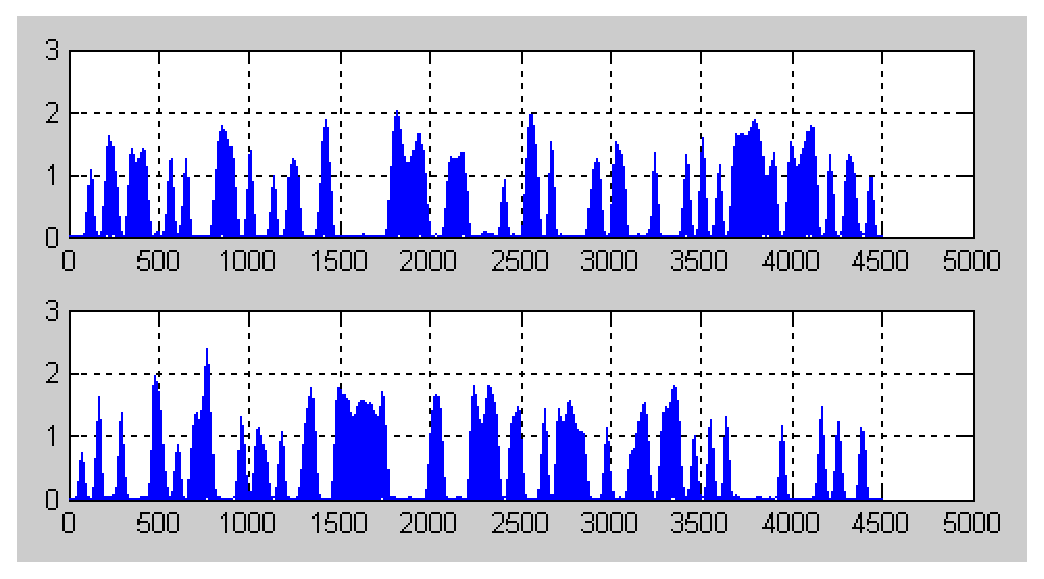
\includegraphics[width=8cm]{bilder/empfaenger/Quadriertessig}
	\caption{Bandpassgefiltertes und quadriertes Signal}
	\label{fig:Quadriertessig}
\end{figure}

\begin{figure}[ht]
	\centering 
%	\psfrag{06}{$N$}
	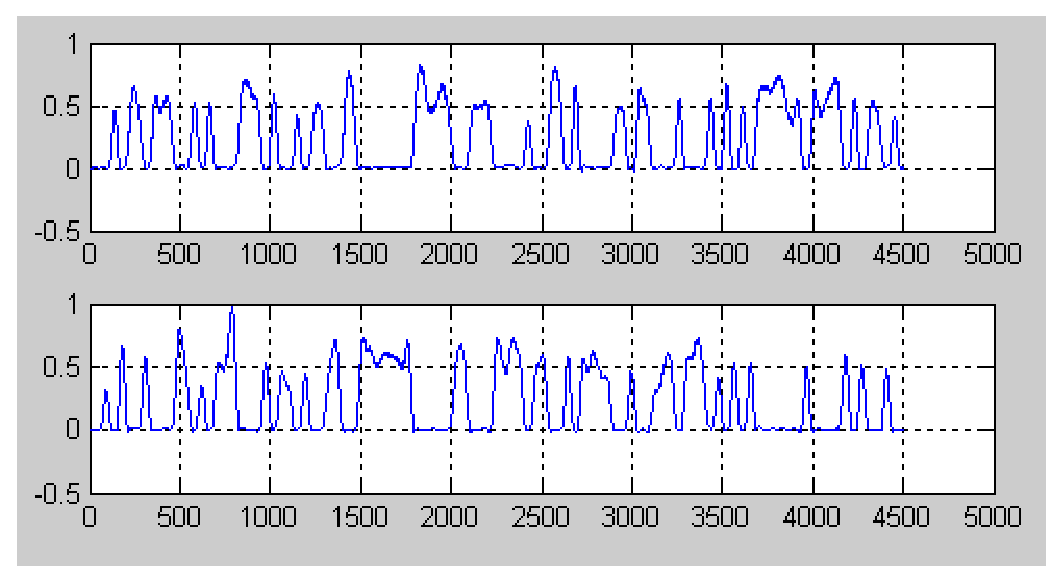
\includegraphics[width=8cm]{bilder/empfaenger/quadutpgefsig}
	\caption{Tiefpassgefiltertes Signal}
	\label{fig:quadutpgefsig}
\end{figure}

Zum Abschluss werden die beiden Signale noch von einander subtrahiert (vgl. Abb. \ref{fig:Empfangssignal}). Im Idealfall sollte das auf diese Weise rekonstruierte Signal dem zu Beginn erzeugten Bitstrom entsprechen.

\begin{figure}[ht]
	\centering 
%	\psfrag{06}{$N$}
	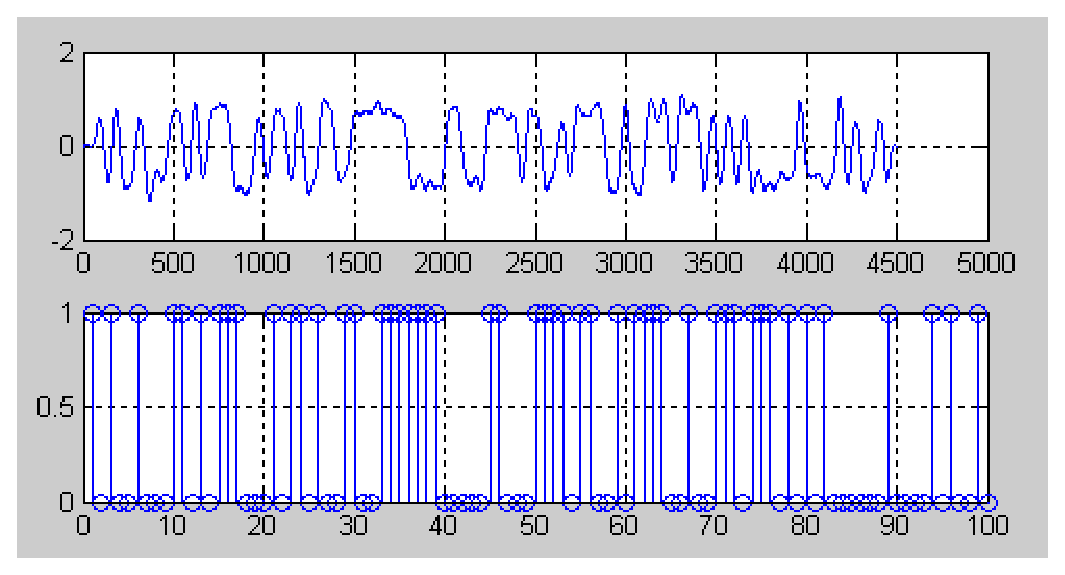
\includegraphics[width=8cm]{bilder/empfaenger/Empfangssig}
	\caption{Rekonstruiertes Empfangssignal}
	\label{fig:Empfangssignal}
\end{figure}

Sie werden nun in den folgenden Kapiteln nach und nach die einzelnen Bl�cke des Empf�ngers selbst entwerfen und die �bertragungsstrecke sowohl als Simulation als auch in Hardware aufbauen.